\chapter{ روش پیشنهادی }
\section{مقدمه}

همان‌طور که در فصل‌ گذشته شرح داده شد، شناسایی چهره در محیط بدون محدودیت به صورت بی‌درنگ و با دقت بالا با چالش‌های بسیاری همراه است. همچنین دقت بالا و زمان پردازش پایین باهم در تقابل هستند. علاوه بر این‌ها، فرض ‌کمبود داده آموزشی نیز چالش بزرگی محسوب می‌شود. بنابراین در این فصل تلاش می‌کنیم تا روشی برای تشخیص دقیق‌تر و بی‌درنگ چهره توسط شبکه عصبی عمیق در تصاویر رنگی پیشنهاد دهیم. در ابتدا مرحله پيش پردازش شرح داده مي‌شود. در قسمت بعد، رويكرد استفاده شده مبتني بر شبكههاي پيچشي به منظور استخراج ویژگی از تصاوير چهره شرح داده خواهد شد. نمای کلی روش ارائه شده در شكل \ref{image4-1} خلاصه شده است كه در ادامه هر يک تشريح خواهد شد. 
\begin{figure}[h]
\centering
  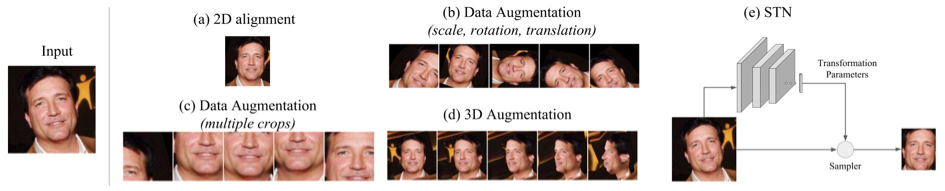
\includegraphics[scale=1]{image3-1}
  \caption{نمای کلی از روش پیشنهادی \cite{ref1}.}
  \label{image4-1}
\end{figure}

\section{پیش پردازش}
بيشتر الگوريتم‌ها‌ي شناسایی چهره نياز به اعمال پيش‌پردازش‌هايي بر روي تصوير ورودي دارند. پیش‌پردازش شامل همسان سازی بافت‌نگار به منظور افزایش تباین، یافتن چهره و تراز کردن تصویر می‌باشد. در ادامه به شرح مراحل پیش‌پردازش می‌پردازیم.
\subsection{همسان سازی بافت‌نگار}
یکی از روش‌های بهبود تصویر، بهبود تباین تصویر است. یکی از روش‌های افزایش تباین تصویر، تکنیک یکنواخت سازی بافت‌نگار است. بطوریکه مقادیر پیکسل‌های تصویر را طوری تغییر می‌دهد تا کل بازه ممکن را تسخیر کند و ایده اساسی آن. نگاشت مقادیر شدت سطوح روشنایی از طریق یک تابع توزیع انتقال است.
این عمل باعث افزایش تباین تصویر  می‌شود که به معنای بهبود کیفیت تصویر و افزایش دقت پردازش های بعدی است. نمونه ای از این روش را از مقاله \cite{s18092995} در شکل \ref{image4-2}  مشاهده می‌نمایید.

\begin{figure}[h]
\centering
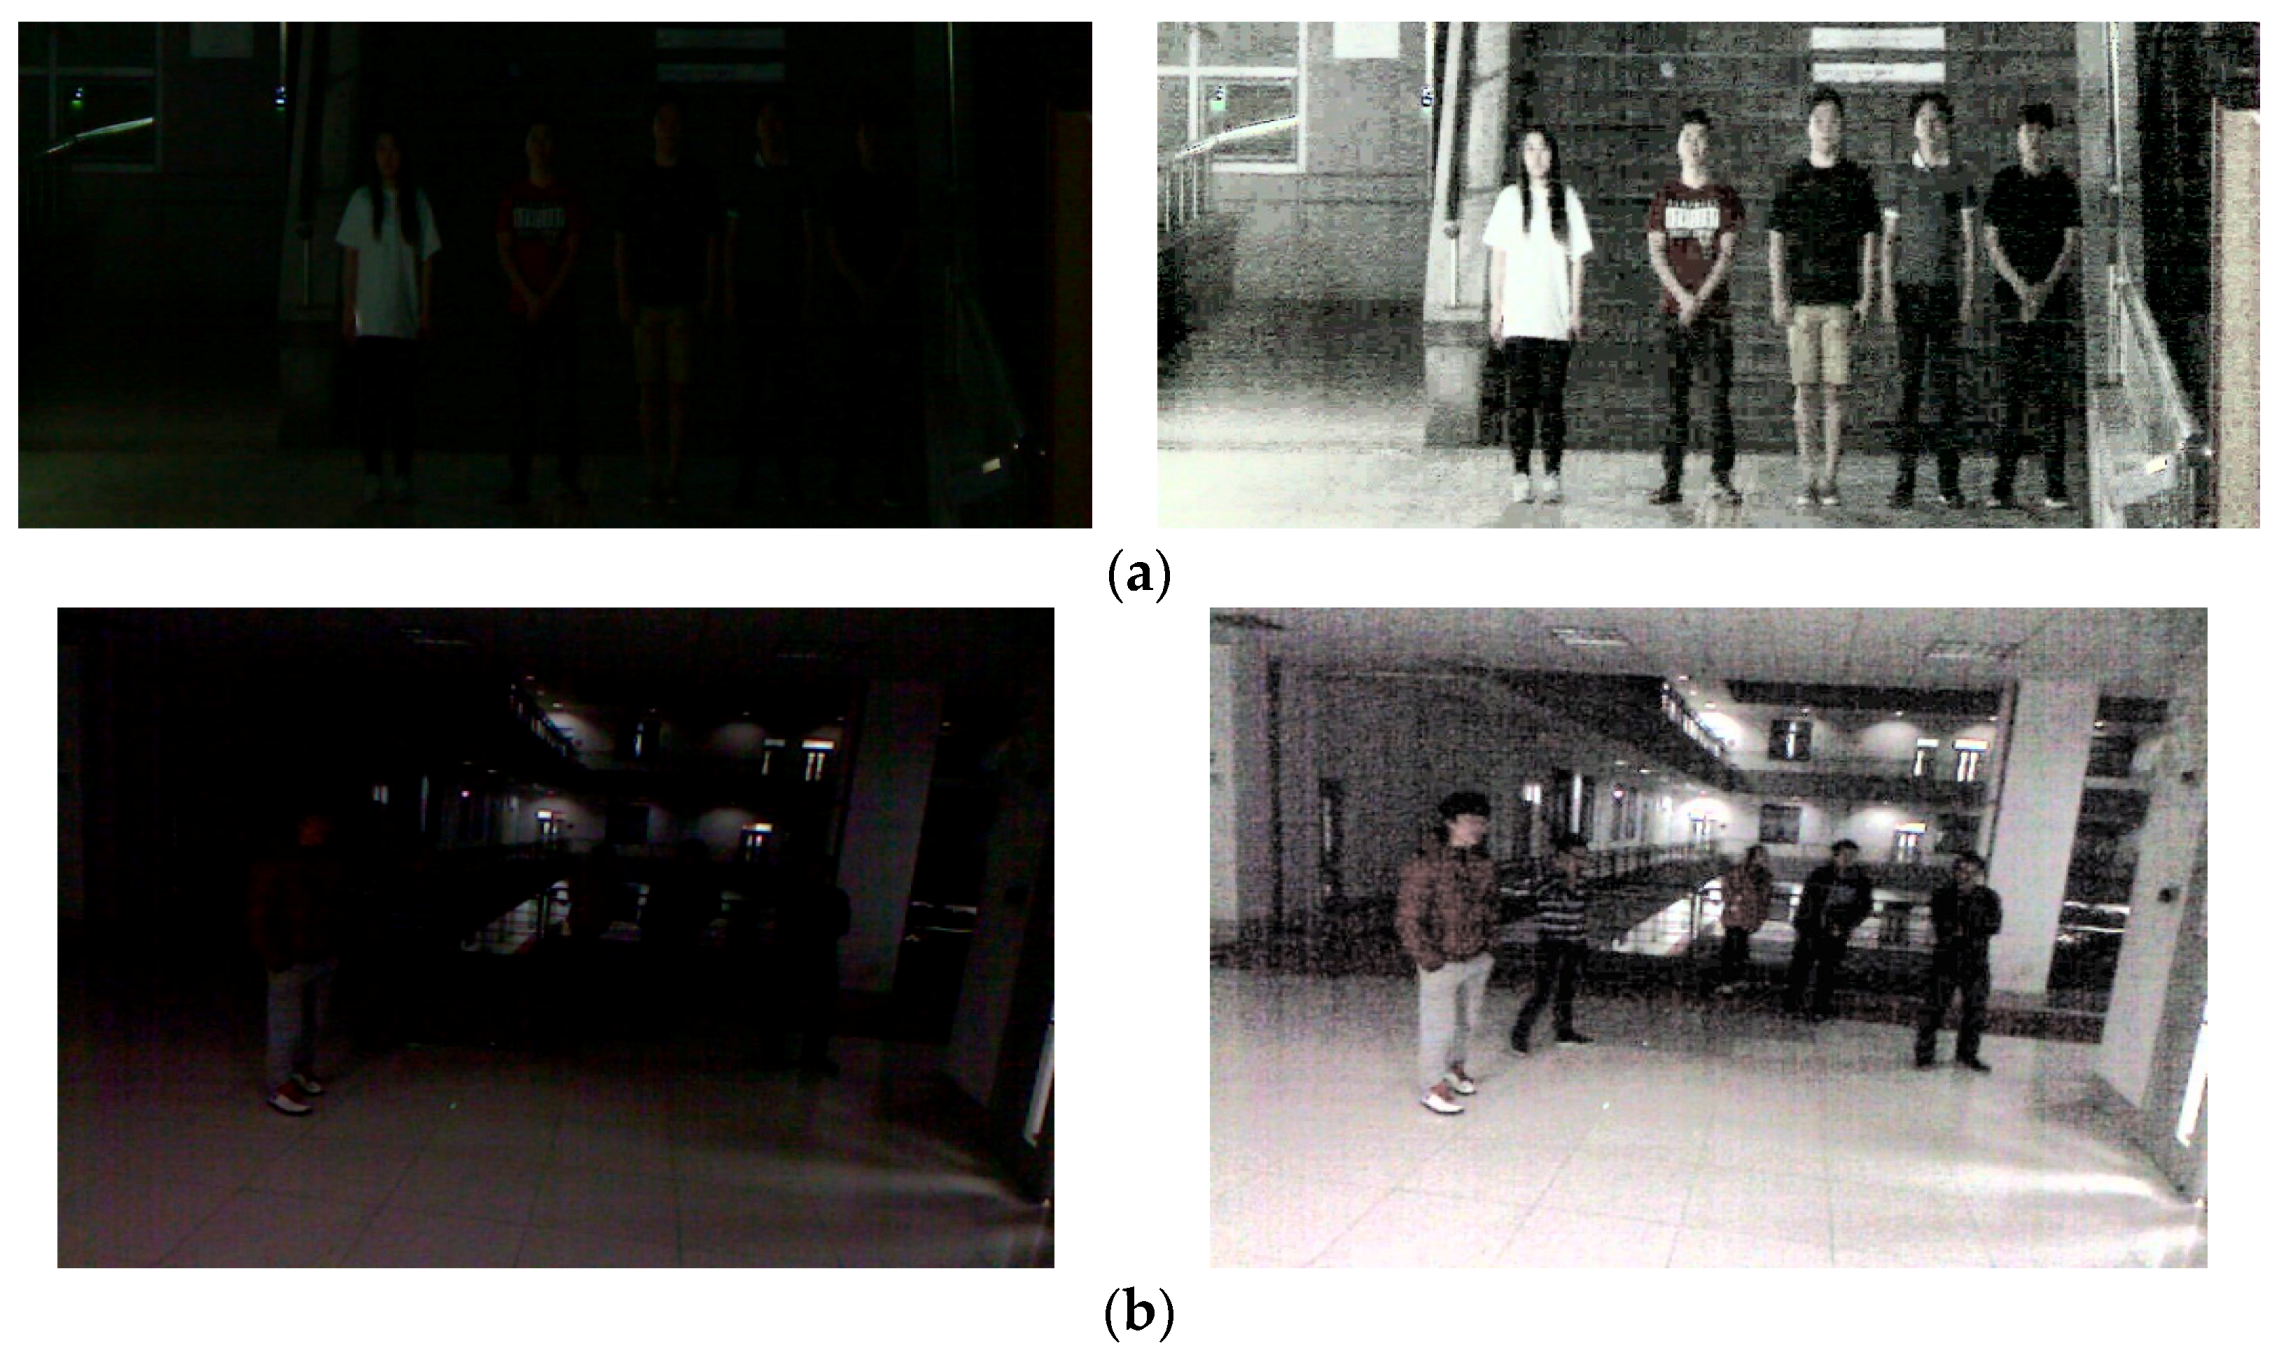
\includegraphics[scale=1]{image4-2}
\caption{نتیجه اعمال یکسان سازی بافت‌نگار بر روی یک تصویر تاریک. تصاویر ورودی در سمت چپ و خروجی در سمت راست می‌باشند \cite{s18092995}.}
\label{image4-2}
\end{figure}

\subsection{یافتن چهره}
يكي ديگر از مراحل معمول پيش پردازش كه در طي فرآيند شناسایی چهره انجام مي‌شود، مکان یابی و یافتن چهره در تصاوير مي‌باشد. برای این منظور از یک روش مبتنی بر شبکه عصبی پیچشی که توسط \lr{Deng} و همکاران \cite{deng2019retinaface} در سال ۲۰۱۹معرفی شده است استفاده می‌کنیم. در این روش برای آموزش شبکه پیچشی از یک تابع ضرر مبتنی بر یادگیری چندکاره استفاده شده است که به صورت زیر می‌باشد.
 \begin{equation}\label{eq3-2}
L = L_cls + L_box + L_pts + L_pixel  
\end{equation}
\noindent
که در آن $L_cls$ تابع ضرر مربوط به یافتن یا عدم یافتن چهره می‌باشد. $L_box$ تابع ضرر مربوط به مکان چهره میباشد. همچنین $L_pts$ تابع ضرر مربوط به یافتن نقاط ویژه روی اجزای چهره می باشد، و $L_pixel$ تابع ضرر مربوط به یافتن یک مدل سه بعدی مبتنی بر مش از روی چهره می باشد. استفاده از تابع ضرر مبتنی بر یادگیری چند کاره کمک می نماید تا فضای مسئله محدود تر شود و الگوریتم مورد نظر زودتر به سمت نقطه بهینه همگرا شود. ما برای رسیدن به خروجی بی درنگ، این روش را بر روی معماری \lr{MobileNetV3} پیاده سازی کرده و آموزش دادیم. نمونه ای از خروجی این روش را در شکل \ref{image4-3} مشاهده می کنید. 
\begin{figure}[h]
\centering
  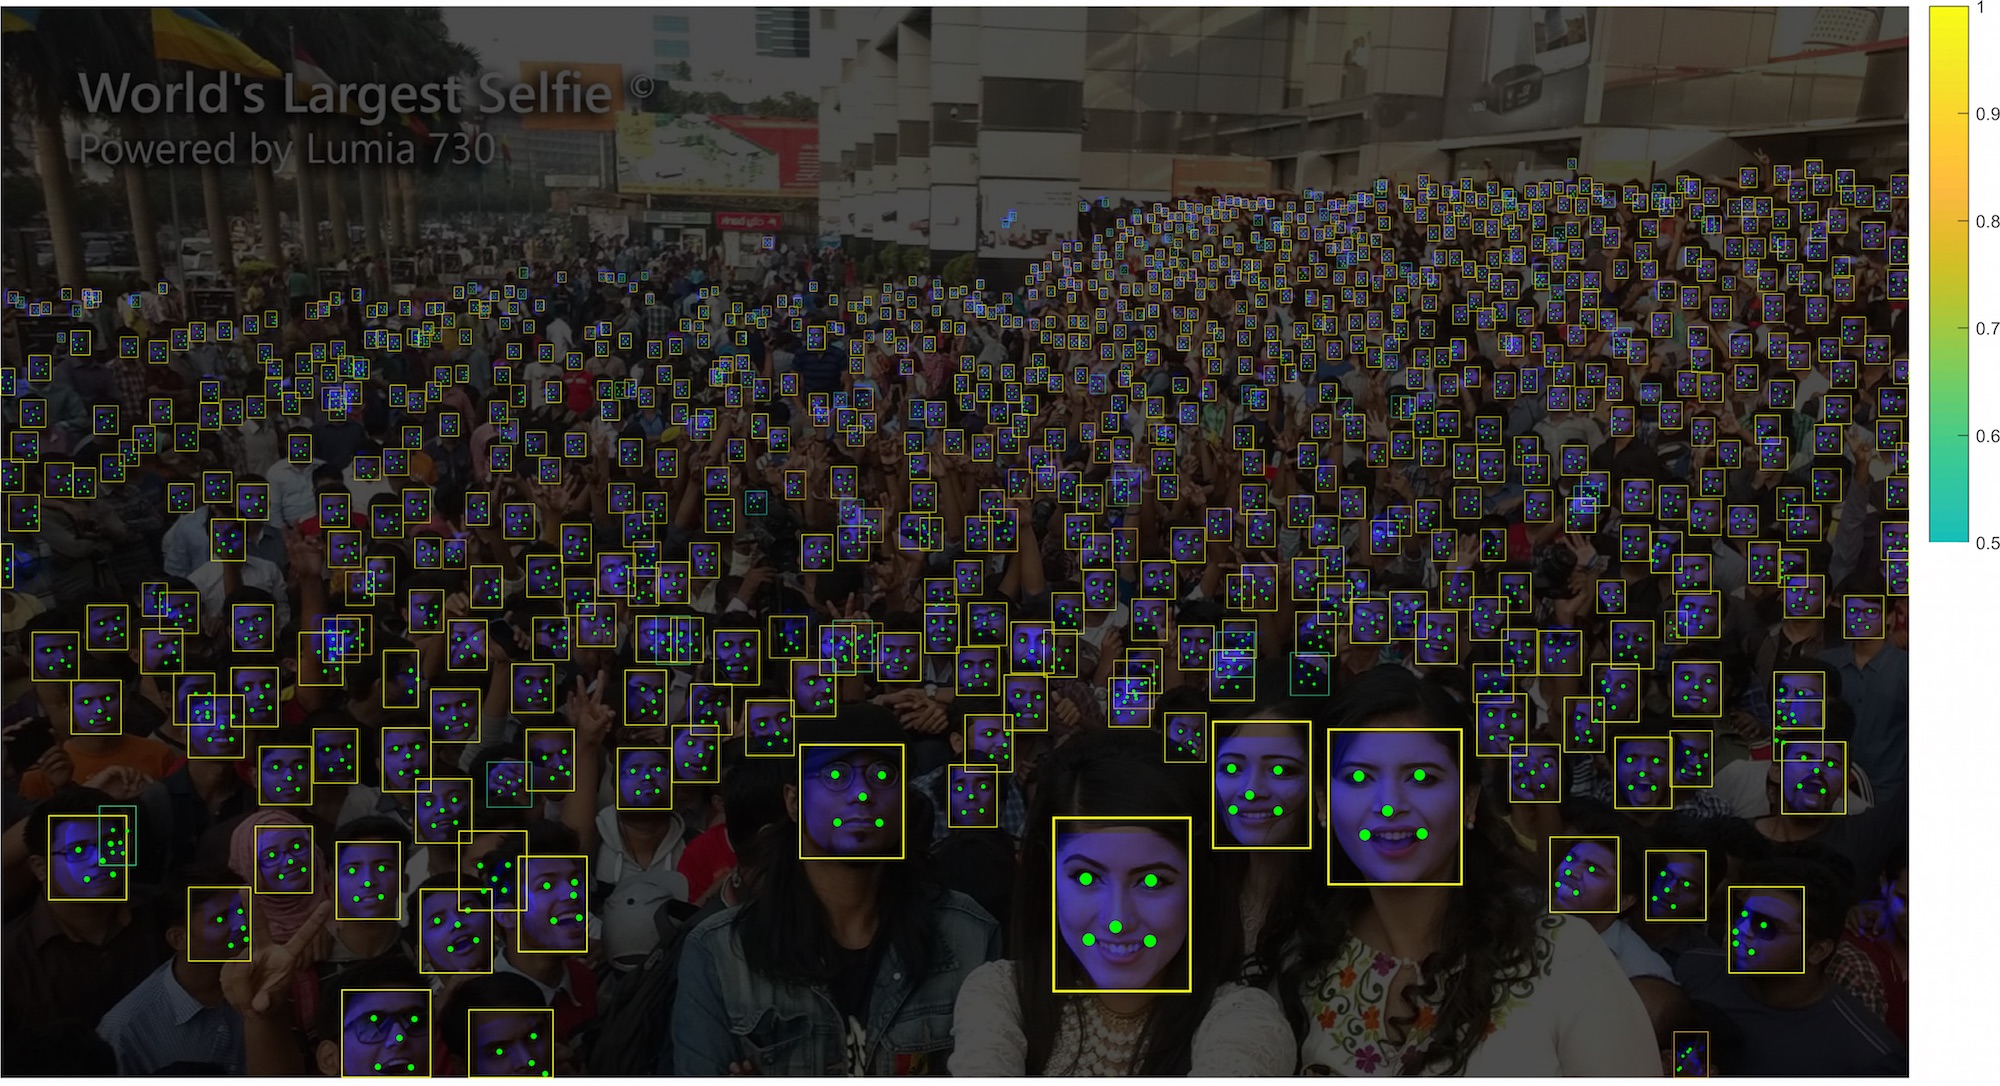
\includegraphics[width=1.0\textwidth]{image4-3}
  \caption{نمونه از خروجی الگوریتم یافتن چهره retina \cite{deng2019retinaface}.}
  \label{image4-3}
\end{figure}

\subsection{تراز کردن تصویر}
در ادامه روند پیش‌پردازش، نوبت به تراز کردن تصویر چهره \LTRfootnote{Face Alignment} می‌رسد. پس از یافتن چهره، به تصویر ورودی مناسب شبکه نزدیک تر می،شویم اما پس از تراز کردن تصویر جهت آموزش شبکه، بهبود دفت نهایی مشهود است. 
بدین منظور با استفاده از یک تبدیل غیرخطی، تصویر چهره را به گونه ای بچرخانیم که چشم،ها در راستای خط افقی قرار بگیرند.
روش‌های کلی برای تشخیص چهره از زاویه‌ی روبه‌رو به خوبی عمل می‌کنند اما مقاومت این روش‌ها در مقابل تغییرات زاویه مناسب نیست، به این علت که ویژگی‌های ظاهری با تغییرات زاویه بسیار تغییر پذیر هستند. با هم‌تراز  کردن تصاویر چهره  با یک تصویر مرجع، پیش از اعمال طبقه‌بند می‌توان تا حدی این مشکل را بهبود داد. در طول هم‌تراز کردن تصویر، نقاط خاصی از تصویر (مانند نقطه‌ی وسط دو چشم و نقاط دو طرف دهان) در نظر گرفته می‌شود و به مختصات مشخصی منتقل می‌شوند. برای این منظور از ۵ نقطه ویژه استخراج شده در مرحله یافتن چهره توسط الگوریتم retina استفاده می‌کنیم. نتیجه اعمال این فرآیند را در شکل \ref{image4-4} مشاهده می‌کنید.

\begin{figure}[h]
\centering
  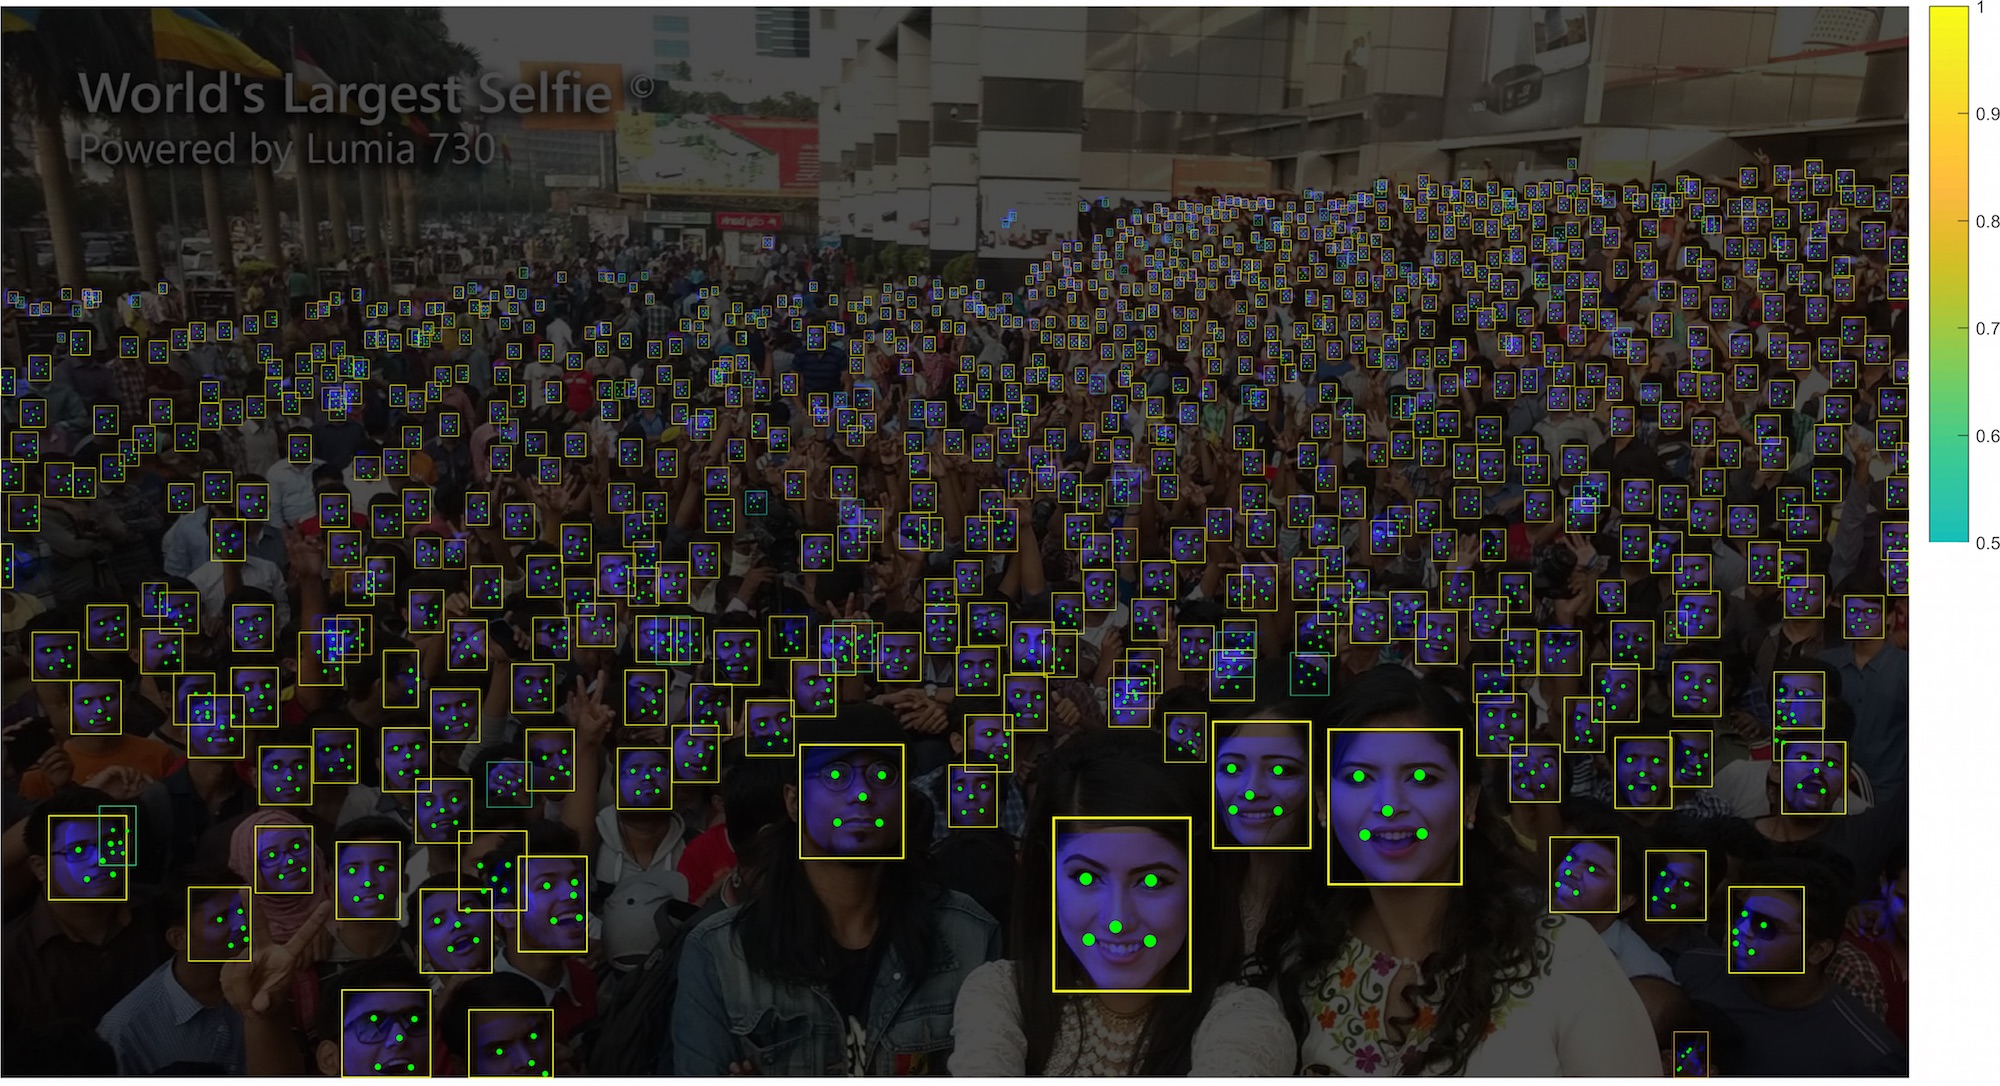
\includegraphics[width=1.0\textwidth]{image4-3}
  \caption{نمونه از خروجی الگوریتم یافتن چهره retina \cite{deng2019retinaface}.}
  \label{image4-4}
\end{figure}

\section{دسته بندی}
روش پیشنهادی برای تشخیص چهره به صورت بی درنگ در محیط های بدون محدودیت، یک الگوریتم مبتنی بر شبکه های پیچشی می‌باشد. این فرایند را می توان به صورت یک مسئله بهینه سازی فرموله کرد که در ادامه به بخش های مختلف آن می پردازیم.

\subsection{مدل پيشنهادي پايه}
ابتدا نوبت آن است که معماری مناسب شبکه برای مسئله را به دست آوریم. با بررسی شبکه‌های به‌روز از جمله
\lr{MobileNetV2},
\lr{MobileNetV3},
\lr{NASNetMobile},
\lr{SqueezeNet},
\lr{VGG19}،
\lr{ResNet-50}،
و
\lr{EfficientNetB0}
و مقایسه دقت و زمان پاسخگویی آن‌ها به کمک یادگیری انتقال، به این نتیجه می‌رسیم که شبکه های \lr{MobileNetV3} و \lr{SqueezeNet} دارای چگالی دقت بالاتری می‌باشند و نسبت دقت دسته بندی به تعداد پارامترهای شبکه در آن‌ها بیشتر می‌باشد. بنابرین می‌تواند سرعت اجرای مناسب و همچنین دقت مناسب را از آن‌ها انتظار داشت. نتایج بررسی را در شکل زیر آمده اند.

آزمایش‌هایی بر روی معماری های مطرح دیگر نیز انجام شد که به علت ضعیف بودن نتایج یا بالا بودن زمان پاسخ دهی در شکل درج نشده‌اند. از نتایج در می یابیم که بهترین معماری شبکه برای مسئله ما معماری \lr{MobileNetV3} است.
\noindent
در این معماری مسير استخراج ويژگي از پنج لايه كانولوشن، چهار لايه خطي و نرمال ساز چهار لايه ديكانولوشن۳ و شش ماژول  تشکیل شده است، كه در ادامه توضيح داده خواهد شد، تصوير ورودي I به بخش استخراج ويژگي داده ميشود و مدل در اين مسير به طور خودكار يك سلسله مراتب ويژگي را از تصاوير ورودي آموزش خواهد ديد و در نهايت اين ويژگيهاي استخراج شده از لايههاي مختلف با يكديگر تركيب شده و به عنوان ورودي تقسيمبند مورد استفاده قرار ميگيرد ]۱۴[ .
\noindent
لايه كانولوشن
سه لايه كانولوشن همراه با گام دو، اندازه حجم ورودي را با ضريبي از دو كاهش ميدهد. سايز پنجره فيلترها 3 × 3 ميباشد. دليل انتخاب سايز كوچك پنجره فيلترها كاهش پيچيدگي محاسباتي و همچنين عملكرد خوب آنها در استخراج ويژگي ميباشد. چگونگي عملكرد يك لايه كانولوشن از رابطه ۲.۳ بدست
ميآيد.
 \begin{figure}[h]
\centering
  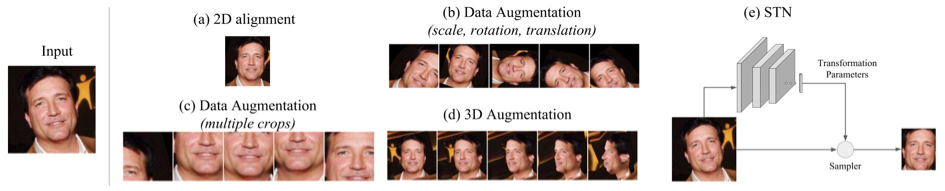
\includegraphics[scale=1]{image3-1}
  \caption{رویکردهای مختلف هم ترازی چهره \cite{ref1}.}
  \label{image2-1}
\end{figure}


\subsection{آموزش شبکه جهت استخراج ویژگی}
از آن‌جایی که ‌شبکه MobileNet معماری بسیار سبک تری نسبت به معماری های شناخته شده دیگر که در فصل ۲ معرفی شدند، دارد؛ بنابراین استخراج ویژگی‌ها از چهره و دسته بندی تصاویر چهره با دقت بالا برای این شبکه بسیار سخت و دشوار است. همچنین در مواردی شباهت چهره افراد به یکدیگر ‌کار را از آن‌چه هست سخت‌تر خواهد کرد. بنابراین ما روشی برای استخراج ویژگی از تصاویر چهره پیشنهاد کرده‌ایم که کمک می‌کند ویژگی‌های استخراج شده که متعلق به دو دسته متفاوت هستند، فاصله بیشتری از هم داشته باشند و در مقابل ویژگی های استخراج شده برای دو تصویر از چهره یک فرد یکسان، فاصله کمتری از هم داشته باشند؛ تا از این طریق بتوان به کاهش مشکلات ذکر شده کمک کرد. این روش شامل بخش‌های تولید چهره، یافتن چهره، آموزش شبکه عصبی پیچشی و ‌استخراج ویژگی می‌باشد.

همانطور که پیش‌تر بیان شد به آموزش این شبکه می‌پردازیم. مجموعه داده خود را پس از پیش‌پردازش و افزایش‌ داده‌ها، آماده می‌کنیم. تعداد کل داده‌های آموزش برای این مرحله را به حدود 320000 رساندیم و آموزش را در 30 دوره انجام داده‌ایم.
\subsection{تابع ضرر}
یکی از چالش های اصلی در یادگیری ویژگی ها با استفاده از شبکه های عصبی عمیق پیوسته \lr{(DCNN)} برای شناسایی چهره در مقیاس بزرگ، طراحی تابع ضرر مناسب است که قدرت تفکیک را افزایش می‌دهد. هدف ما کم کردن فاصله بین ویژگی‌های عمیق و مراکز کلاس‌های آن‌ها در فضای اقلیدسی برای دستیابی به فشردگی درون کلاسی بیشتر می‌باشد. ما یک تابع ضرر برای افزایش زاویه ای حاشیه برای دستیابی به ویژگی های بسیار متمایز برای تشخیص چهره پیشنهاد می‌کنیم که عملکرد بهتر برخوردار است و می توان آن را به راحتی با هزینه های محاسباتی ناچیز پیاده سازی کرد.
\noindent
برای آموزش شبکه های عصبی عمیق پیوسته برای تشخیص چهره، دو رویکرد اصلی وجود دارد. روش اول دسته بندی را آموزش می دهند که می تواند هویت های مختلف را در مجموعه آموزش از هم جدا کند، مانند با استفاده از طبقه بندی \lr{softmax}، و رویکرد دوم که مستقیماً یک تعبیه را یاد می گیرند، مانند \lr{triplet loss}. بر اساس داده های آموزش در مقیاس بزرگ و معماری \lr{DCNN}، هر دو روش می توانند عملکرد بسیار خوبی در تشخیص چهره داشته باشند. با این حال، هم رویکرد \lr{softmax} و هم رویکرد \lr{triplet loss} اشکالاتی دارد.
\noindent
برای :
\begin{enumerate}
\item
	اندازه ماتریس تبدیل W به طور خطی با افزایش تعداد دسته ها \lr{(n)} افزایش می یابد.‌
\item 
ویژگیهای آموخته شده برای مسئله‌های طبقه بندی با مجموعه بسته قابل تفکیک هستند اما به اندازه کافی برای مسئله تشخیص چهره که یک مسئله باز می‌باشد، مناسب نیستند. 
\end{enumerate}
\noindent
برای \lr{triplet loss}:
\begin{enumerate}
\item
 برای مجموعه داده های مقیاس بزرگ، رشد شدید در تعداد ترکیب‌های تعداد تصاویر سه گانه وجود دارد که منجر به افزایش قابل توجه تعداد مراحل تکرار می‌شود.
\item 
 استخراج مجموعه تصاویر سه گانه یک مسئله دشوار برای آموزش موثر می‌باشد. 
\end{enumerate}
\noindent
ما برای افزایش بیشتر قدرت تمایز مدل تشخیص چهره و ایجاد ثبات در روند آموزش، تابع ضرر مبتنی بر توابع مثلثاتی را پیشنهاد می‌کنیم. همانطور که در شکل 2 نشان داده شده است، حاصل ضرب نقطه ای مقادیر موجود در ویژگی های استخراج شده و آخرین لایه کاملاً متصل، برابر با ضرب کسینوسی آن‌ها پس از نرمال سازی می باشد‌، ما از تابع مثلثاتی کسینوسی برای محاسبه زاویه بین ویژگی فعلی و وزن هدف استفاده می‌کنیم. سپس یک حاشیه زاویه ای به زاویه هدف اضافه می‌کنیم‌، در انتها با استفاده از تابع کسینوس دوباره مقادیر را به فضای خطی برمی‌گردانیم. مراحل بعدی دقیقاً مانند \lr{softmax} هستند.
مزایای این روش پیشنهادی را می‌توان به شرح زیر خلاصه کرد:
\begin{itemize}
 \item
در مجموعه داده های تصویر و فیلم در مقیاس بزرگ ، به عملکرد مناسبی دست می یابد.
 \item
فقط به چندین خط کد نیاز دارد و اجرای آن در چارچوب های یادگیری عمیق مبتنی بر \lr{Pytorch} و \lr{Tensorflow} آسان است. برای داشتن عملکرد پایدار نیازی به ترکیب با سایر توابع ضرر ندارد و به راحتی همگرا می‌شود.
 \item
هنگام آموزش فقط پیچیدگی محاسباتی ناچیز را اضافه می کند. پردازنده های گرافیکی کنونی می توانند به راحتی از هزاران دسته مختلف برای آموزش پشتیبانی کنند و مدل به راحتی می تواند هویت های بیشتری را پشتیبانی کند.
\end{itemize} 
\noindent


رابطه ریاضی \lr{softmax} معروف ترین تابع ضرر طبقه بندی که به طور گسترده استفاده می شود، به شرح زیر است:
\begin{equation}\label{eq4-1}
L= - \frac{1}{N} \sum_{i=1}^{N} log \frac{e^{{W_{y_i}^T} x_i + b_{y_i}}}{\sum_{j=1}^{n} e^{{W_j^T} x_i + b_j}} 
\end{equation}
\noindent
که در آن \lr{xi} نشان دهنده ویژگی عمیق نمونه \lr{i} ازدسته \lr{y} است. تعداد ابعاد ویژگی استخراج شده را 512 در نظر گرفتیم. \lr{Wj} ستون \lr{j}  ام از وزن \lr{W} می‌باشد و \lr{bj} بایاس است. مقدار \lr{N}اندازه دسته و \lr{n} تعداد دسته‌ها است. این تابع مستقیما ویژگی استخراج شده را برای اعمال شباهت بالاتر برای نمونه های درون کلاس و فاصله بیشتر برای نمونه های بین کلاسی بهینه نمی‌کند، که منجر به ایجاد مشکل در عملکرد آن برای تشخیص چهره عمیق تحت تغییرات ظاهری بزرگ درون کلاس می شود (به عنوان مثال تغییرات زاویه چهره و تقییرات سنی).

\noindent
ما رابطه فوق را مبنای محاسبات قرار دادیم و تغییرات جزیی به آن اضافه کردیم. برای سادگی مقدار بایاس را صفر در نظر گرفتیم. سپس حاصل ضرب مقادیر موجود در ویژگی های استخراج شده و آخرین لایه کامل
متصل را به صورت
$W_j^T x_i = ||W_j|| ||x_i|| cos(θ_j)$
تبدیل می کنیم، که \lr{θj} زاویه بین وزن \lr{Wj} و ویژگی \lr{xi} است. نرمال سازی ویژگی‌ها و وزن‌ها باعث می‌شود که خروجی فقط به زاویه بین ویژگی و وزن بستگی داشته باشد. به کمک نرمال سازی مقادیر وزن $||W_j||$ را برابر ۱ در نظر می‌گیریم. همچنین ویژگی استخراج شده $||x_i||$ را نرمال کرده و نام آن را \lr{s} در نظر می‌گیریم. ‌‌‌بنابرین ویژگی‌های استخراج شده در یک ابر کره با شعاع s توزیع می‌شوند. برای افزایش حاشیه بین \lr{xi} و \lr{Wj} یک مقدار \lr{m}اضافه می‌کنیم تا به طور همزمان فشرده سازی درون کلاسی و اختلاف بین کلاسی را افزایش دهیم.
\begin{equation}\label{eq4-2}
L = - \frac{1}{N} \sum_{i=1}^{N} log \frac{e^{s(cos(\theta_{y_i}+m))}}{e^{s(cos(\theta_{y_i}+m))} + \sum_{j=1}^{n} e^{s(cos(\theta_j))}}
\end{equation}
\noindent
همانطور که در شکل 3 نشان داده شده است، \lr{softmax} ویژگی‌های تقریباً قابل تفکیکی ایجاد می‌کند اما در مرزهای تصمیم گیری ابهام قابل توجهی به وجود می‌آید، در حالی که تابع ضرر ما می تواند فاصله بیشتری را بین دسته‌های نزدیک اعمال کند.
\begin{figure}[h]
\centering
  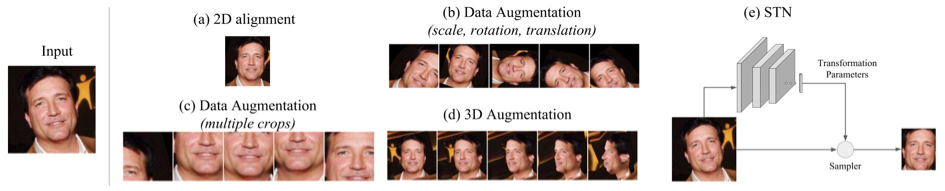
\includegraphics[scale=1]{image3-1}
  \caption{رویکردهای مختلف هم ترازی چهره \cite{ref1}.}
  \label{image2-1}
\end{figure}


\subsubsection{آموزش‌}
در ابتداي روند آموزش، لازم است پارامترهاي مدل مقدار دهي اوليه شوند و انتخاب پارامترهاي اوليه ميتواند تأثير زيادي در مدل آموزش يافته داشته باشد. در اين پژوهش به منظور مقدار دهي اوليه پارامترها از تابع توزيع يكنواخت استفاده شده است. از ديگر چالشهاي اساسي براي روشهاي بهينه سازي مبتني بر گراديان، انتخاب ميزان نرخ يادگيري مناسب است. روشهاي كلاسيك گراديان تصادفي از نرخ يادگيري ثابت يا كاهشي استفاده ميكنند، كه براي همه پارامترهاي مدل يكسان است. با اين حال، مشتقات جزئي پارامترهاي لايههاي مختلف ميتوانند از نظر مقدار متفاوت باشند، كه ميتواند به نرخ يادگيري مختلفي نياز داشته باشد. با اين حال، مشتقات جزئي پارامترهاي لايههاي مختلف ميتوانند از نظر مقدار تفاوت قابل توجهي داشته باشند، كه ميتواند به نرخ يادگيري مختلفي نياز داشته باشد. در سالهاي اخير، تمايل به توسعه روشهايي براي انتخاب خودكار نرخ يادگيري مستقل افزايش يافته است. اكثر روشها )به عنوان مثال، RMSprop، [۴۸]AdaDelta، [۴۷]AdaGrad]۴۹[ و Adam]۵۰[( آمارهاي مختلف مشتقات جزئي را در چندين تكرار جمع آوري ميكنند و از اين اطلاعات براي تعيين ميزان يادگيري سازگار براي هر پارامتر استفاده ميكنند. اين امر به ويژه براي آموزش شبكههاي عميق بسيار مهم است، جايي كه نرخ يادگيري مطلوب اغلب براي هر لايه بسيار متفاوت است. در اين پژوهش در آزمايشات انجام شده از همه روشهاي نام برده استفاده شد ولي روش Adam عملكرد بهتري ارائه داده است.

\subsubsection{دسته‌بندی}
در مرحله آزمون به منظور تشخیص هویت یک تصویر چهره، پس از پیش‌پردازش تصویر را مطابق با ورودی شبکه تغییر اندازه میدهیم و جهت استخراج ویژگی‌ به آن شبکه می‌دهیم. پس از استخراج ویژگی ها توسط شبکه، بردار ۵۱۲ تایی بدست آمده را با بردار های مربوط به چهره های بانک اطلاعاتی مقایسه کرده و با محاسبه فاصله اقلیدسی بردار ها، نزدیک ترین شخص مورد نظر انتخاب شده و در صورتی که فاصله میان بردار ویژگی آن ها از حد آستانه کمتر باشد. عمل دسته بندی انجام شده و هویت چهره مورد نظر تعیین می شود. در غیر این صورت اعلام میداریم که شخص مورد نظر قابل شناسایی نمی باشد.

\begin{figure}[h]
\centering
  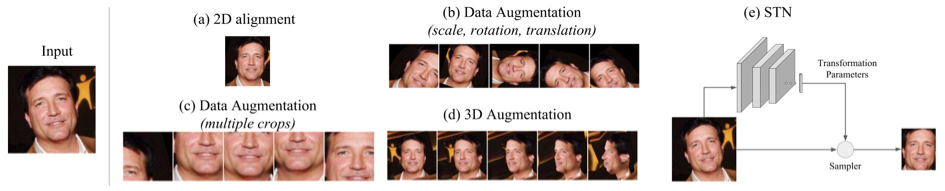
\includegraphics[scale=1]{image3-1}
  \caption{رویکردهای مختلف هم ترازی چهره \cite{ref1}.}
  \label{image2-1}
\end{figure}

\section{فناوری های استفاده شده}
پیاده‌سازی این الگوریتم به کمک زبان برنامه‌ نویسی پایتون و کتابخانه \lr{PyTorch} و \lr{OpenCV}انجام شده است. از کتابخانه‌های مهم مورد استفاده دیگر در این کار می‌‌توان به \lr{NumPy} برای انجام محاسبات ماتریسی و \lr{SciPy} و \lr{Scikit Learn} اشاره کرد.[35] 

برای آموزش شبکه عصبی مربوط به دسته بندی ۱۲ گیگابایت حافظه اصلی و ۱۲ گیگابایت حافظه گرافیکی در اختیار گرفتیم.
